% Options for packages loaded elsewhere
\PassOptionsToPackage{unicode}{hyperref}
\PassOptionsToPackage{hyphens}{url}
\PassOptionsToPackage{dvipsnames,svgnames,x11names}{xcolor}
%
\documentclass[
]{article}
\usepackage{amsmath,amssymb}
\usepackage{iftex}
\ifPDFTeX
  \usepackage[T1]{fontenc}
  \usepackage[utf8]{inputenc}
  \usepackage{textcomp} % provide euro and other symbols
\else % if luatex or xetex
  \usepackage{unicode-math} % this also loads fontspec
  \defaultfontfeatures{Scale=MatchLowercase}
  \defaultfontfeatures[\rmfamily]{Ligatures=TeX,Scale=1}
\fi
\usepackage{lmodern}
\ifPDFTeX\else
  % xetex/luatex font selection
\fi
% Use upquote if available, for straight quotes in verbatim environments
\IfFileExists{upquote.sty}{\usepackage{upquote}}{}
\IfFileExists{microtype.sty}{% use microtype if available
  \usepackage[]{microtype}
  \UseMicrotypeSet[protrusion]{basicmath} % disable protrusion for tt fonts
}{}
\makeatletter
\@ifundefined{KOMAClassName}{% if non-KOMA class
  \IfFileExists{parskip.sty}{%
    \usepackage{parskip}
  }{% else
    \setlength{\parindent}{0pt}
    \setlength{\parskip}{6pt plus 2pt minus 1pt}}
}{% if KOMA class
  \KOMAoptions{parskip=half}}
\makeatother
\usepackage{xcolor}
\usepackage[margin=1in]{geometry}
\usepackage{color}
\usepackage{fancyvrb}
\newcommand{\VerbBar}{|}
\newcommand{\VERB}{\Verb[commandchars=\\\{\}]}
\DefineVerbatimEnvironment{Highlighting}{Verbatim}{commandchars=\\\{\}}
% Add ',fontsize=\small' for more characters per line
\usepackage{framed}
\definecolor{shadecolor}{RGB}{248,248,248}
\newenvironment{Shaded}{\begin{snugshade}}{\end{snugshade}}
\newcommand{\AlertTok}[1]{\textcolor[rgb]{0.94,0.16,0.16}{#1}}
\newcommand{\AnnotationTok}[1]{\textcolor[rgb]{0.56,0.35,0.01}{\textbf{\textit{#1}}}}
\newcommand{\AttributeTok}[1]{\textcolor[rgb]{0.13,0.29,0.53}{#1}}
\newcommand{\BaseNTok}[1]{\textcolor[rgb]{0.00,0.00,0.81}{#1}}
\newcommand{\BuiltInTok}[1]{#1}
\newcommand{\CharTok}[1]{\textcolor[rgb]{0.31,0.60,0.02}{#1}}
\newcommand{\CommentTok}[1]{\textcolor[rgb]{0.56,0.35,0.01}{\textit{#1}}}
\newcommand{\CommentVarTok}[1]{\textcolor[rgb]{0.56,0.35,0.01}{\textbf{\textit{#1}}}}
\newcommand{\ConstantTok}[1]{\textcolor[rgb]{0.56,0.35,0.01}{#1}}
\newcommand{\ControlFlowTok}[1]{\textcolor[rgb]{0.13,0.29,0.53}{\textbf{#1}}}
\newcommand{\DataTypeTok}[1]{\textcolor[rgb]{0.13,0.29,0.53}{#1}}
\newcommand{\DecValTok}[1]{\textcolor[rgb]{0.00,0.00,0.81}{#1}}
\newcommand{\DocumentationTok}[1]{\textcolor[rgb]{0.56,0.35,0.01}{\textbf{\textit{#1}}}}
\newcommand{\ErrorTok}[1]{\textcolor[rgb]{0.64,0.00,0.00}{\textbf{#1}}}
\newcommand{\ExtensionTok}[1]{#1}
\newcommand{\FloatTok}[1]{\textcolor[rgb]{0.00,0.00,0.81}{#1}}
\newcommand{\FunctionTok}[1]{\textcolor[rgb]{0.13,0.29,0.53}{\textbf{#1}}}
\newcommand{\ImportTok}[1]{#1}
\newcommand{\InformationTok}[1]{\textcolor[rgb]{0.56,0.35,0.01}{\textbf{\textit{#1}}}}
\newcommand{\KeywordTok}[1]{\textcolor[rgb]{0.13,0.29,0.53}{\textbf{#1}}}
\newcommand{\NormalTok}[1]{#1}
\newcommand{\OperatorTok}[1]{\textcolor[rgb]{0.81,0.36,0.00}{\textbf{#1}}}
\newcommand{\OtherTok}[1]{\textcolor[rgb]{0.56,0.35,0.01}{#1}}
\newcommand{\PreprocessorTok}[1]{\textcolor[rgb]{0.56,0.35,0.01}{\textit{#1}}}
\newcommand{\RegionMarkerTok}[1]{#1}
\newcommand{\SpecialCharTok}[1]{\textcolor[rgb]{0.81,0.36,0.00}{\textbf{#1}}}
\newcommand{\SpecialStringTok}[1]{\textcolor[rgb]{0.31,0.60,0.02}{#1}}
\newcommand{\StringTok}[1]{\textcolor[rgb]{0.31,0.60,0.02}{#1}}
\newcommand{\VariableTok}[1]{\textcolor[rgb]{0.00,0.00,0.00}{#1}}
\newcommand{\VerbatimStringTok}[1]{\textcolor[rgb]{0.31,0.60,0.02}{#1}}
\newcommand{\WarningTok}[1]{\textcolor[rgb]{0.56,0.35,0.01}{\textbf{\textit{#1}}}}
\usepackage{graphicx}
\makeatletter
\def\maxwidth{\ifdim\Gin@nat@width>\linewidth\linewidth\else\Gin@nat@width\fi}
\def\maxheight{\ifdim\Gin@nat@height>\textheight\textheight\else\Gin@nat@height\fi}
\makeatother
% Scale images if necessary, so that they will not overflow the page
% margins by default, and it is still possible to overwrite the defaults
% using explicit options in \includegraphics[width, height, ...]{}
\setkeys{Gin}{width=\maxwidth,height=\maxheight,keepaspectratio}
% Set default figure placement to htbp
\makeatletter
\def\fps@figure{htbp}
\makeatother
\setlength{\emergencystretch}{3em} % prevent overfull lines
\providecommand{\tightlist}{%
  \setlength{\itemsep}{0pt}\setlength{\parskip}{0pt}}
\setcounter{secnumdepth}{-\maxdimen} % remove section numbering
\ifLuaTeX
  \usepackage{selnolig}  % disable illegal ligatures
\fi
\IfFileExists{bookmark.sty}{\usepackage{bookmark}}{\usepackage{hyperref}}
\IfFileExists{xurl.sty}{\usepackage{xurl}}{} % add URL line breaks if available
\urlstyle{same}
\hypersetup{
  pdftitle={STAT 442: Assignment 1},
  colorlinks=true,
  linkcolor={Maroon},
  filecolor={Maroon},
  citecolor={Blue},
  urlcolor={blue},
  pdfcreator={LaTeX via pandoc}}

\title{STAT 442: Assignment 1}
\usepackage{etoolbox}
\makeatletter
\providecommand{\subtitle}[1]{% add subtitle to \maketitle
  \apptocmd{\@title}{\par {\large #1 \par}}{}{}
}
\makeatother
\subtitle{DUE: Wednesday January 29 by 11:59pm EST}
\author{}
\date{\vspace{-2.5em}}

\begin{document}
\maketitle

\section{Part 1 - Reading: Evaluating Effects of Background Stories on
Graph Perception {[}12 marks, 2 marks
each{]}}\label{part-1---reading-evaluating-effects-of-background-stories-on-graph-perception-12-marks-2-marks-each}

Read the first 7 pages of the article ``Evaluating Effects of Background
Stories on Graph Perception'' by Ying Zhao et al.~and answer the
following questions. Each answer should be at MOST one or two sentences,
and you may copy directly from the source article without citing.

\begin{enumerate}
\def\labelenumi{\alph{enumi})}
\tightlist
\item
  What is the difference between a graph (any type of visualization) and
  a graph (visualization of a network)?
\end{enumerate}

A graph is an abstract model representing relations among entities,
while a graph visualization (e.g., node-link diagram) is a method to
visually represent connections among entities.

\begin{enumerate}
\def\labelenumi{\alph{enumi})}
\setcounter{enumi}{1}
\tightlist
\item
  In the context of this article, what is a UBSer and an FBSer?
\end{enumerate}

UBSers: Viewers unaware of the background story.

FBSers: Viewers aware of the background story.

\begin{enumerate}
\def\labelenumi{\alph{enumi})}
\setcounter{enumi}{2}
\tightlist
\item
  What is one of the three hypotheses that the article explores about
  background stories? (Quoting any one of the three is fine)
\end{enumerate}

H2. Background stories can affect the performance of identifying graph
structures.

\begin{enumerate}
\def\labelenumi{\alph{enumi})}
\setcounter{enumi}{3}
\tightlist
\item
  What is a metric proposed for graph readability?
\end{enumerate}

One metric is the number of edge crossings and edge bends, proposed by
Purchase et al., to measure the aesthetic readability of graph layouts.

\begin{enumerate}
\def\labelenumi{\alph{enumi})}
\setcounter{enumi}{4}
\tightlist
\item
  What is the name that the article uses for the context of the graph
  that is not shown in the graph. In other words, the ``missing
  datapoints that are in our head'', or the ``exformation''?
\end{enumerate}

The article refers to it as ``non-displayed contexts,'' which include
invisible knowledge and experience that influence how viewers perceive
graphs.

\begin{enumerate}
\def\labelenumi{\alph{enumi})}
\setcounter{enumi}{5}
\tightlist
\item
  What are the three types of graph structures that the participants
  were asked to identify in one of the experiments?
\end{enumerate}

The three types are:

\begin{itemize}
\item
  high degree nodes
\item
  bridges
\item
  communities
\end{itemize}

\newpage

\section{Part 2 - Make a tier list {[}16
marks{]}}\label{part-2---make-a-tier-list-16-marks}

(16 marks) A client wants a function to make a tier list in R with text
instead of images. (Credit to Tierzoo)

Make a function called \texttt{tierlist} that does the following:

\begin{itemize}
\tightlist
\item
  Draws a black background with rectangles for each of the tiers
  described by \texttt{tiernames} and \texttt{tiercols}.
\item
  Draws a main title in white text described in \texttt{main} above the
  rectangles.
\item
  Takes in a dataframe \texttt{df} that has a \texttt{tier} variable and
  \texttt{text} variable.
\item
  For each row of \texttt{df}, makes a white box in the appropriate tier
  and fills it with the black text in \texttt{text}.
\item
  Each bar should have room for four boxes, but only filled boxes should
  be draw
\end{itemize}

\begin{Shaded}
\begin{Highlighting}[]
\NormalTok{tierlist }\OtherTok{=} \ControlFlowTok{function}\NormalTok{(df, }\AttributeTok{tiernames=}\FunctionTok{c}\NormalTok{(}\StringTok{"S"}\NormalTok{,}\StringTok{"A"}\NormalTok{,}\StringTok{"B"}\NormalTok{,}\StringTok{"C"}\NormalTok{,}\StringTok{"D"}\NormalTok{,}\StringTok{"F"}\NormalTok{), }
                    \AttributeTok{tiercols =} \FunctionTok{c}\NormalTok{(}\StringTok{"lightblue"}\NormalTok{,}\StringTok{"green"}\NormalTok{, }\StringTok{"lightgreen"}\NormalTok{, }\StringTok{"yellow"}\NormalTok{, }\StringTok{"orange"}\NormalTok{, }\StringTok{"red"}\NormalTok{),}
                    \AttributeTok{main=}\StringTok{"My Tier List"}\NormalTok{) \{}

\NormalTok{  Ntiers }\OtherTok{=} \FunctionTok{length}\NormalTok{(tiernames)}
  \CommentTok{\# Counts number of tiers to be created}

\NormalTok{  tier\_start\_y }\OtherTok{=}\NormalTok{ y\_top }\SpecialCharTok{*} \FloatTok{0.9}
  \CommentTok{\# Starts tiers 10\% from the top of the window}
  
\NormalTok{  tier\_start\_x }\OtherTok{=}\NormalTok{ ((X\_right }\SpecialCharTok{{-}}\NormalTok{ x\_left) }\SpecialCharTok{*} \FloatTok{0.1} \SpecialCharTok{+}\NormalTok{ x\_left)}
  \CommentTok{\# Starts tiers 10\% from the left of the window}

\NormalTok{  space }\OtherTok{=}\NormalTok{ (tier\_start\_y }\SpecialCharTok{{-}}\NormalTok{ y\_bottom) }\SpecialCharTok{/}\NormalTok{ Ntiers}
  \CommentTok{\# Space the tiers have by the number to tiers to ensure they are equal}
  
\NormalTok{  tier\_height }\OtherTok{=}\NormalTok{ space }\SpecialCharTok{*} \FloatTok{0.9}
  \CommentTok{\# Tier height so that there is a gap between tiers}
  
  \FunctionTok{rect}\NormalTok{(x\_left, y\_bottom, X\_right, y\_top, }\AttributeTok{col =} \StringTok{"black"}\NormalTok{)}
  \FunctionTok{text}\NormalTok{((X\_right }\SpecialCharTok{+}\NormalTok{ x\_left) }\SpecialCharTok{/} \DecValTok{2}\NormalTok{, y\_top }\SpecialCharTok{*} \FloatTok{0.95}\NormalTok{, }\AttributeTok{labels =}\NormalTok{ main, }\AttributeTok{col =} \StringTok{"white"}\NormalTok{)}
  \CommentTok{\# Draws the background and created the title }
  
  \ControlFlowTok{for}\NormalTok{ (i }\ControlFlowTok{in} \DecValTok{1}\SpecialCharTok{:}\NormalTok{Ntiers) \{}
\NormalTok{    this\_df }\OtherTok{=} \FunctionTok{subset}\NormalTok{(df, tier }\SpecialCharTok{==}\NormalTok{ tiernames[i])}
\NormalTok{    Nboxes }\OtherTok{=} \FunctionTok{nrow}\NormalTok{(this\_df)}

    \ControlFlowTok{if}\NormalTok{ (i }\SpecialCharTok{\textgreater{}} \DecValTok{1}\NormalTok{) \{}
\NormalTok{      tier\_start\_y }\OtherTok{=}\NormalTok{ tier\_start\_y }\SpecialCharTok{{-}}\NormalTok{ space}
      \CommentTok{\#changes the y for the second and so on tiers}
\NormalTok{    \}}

    \FunctionTok{rect}\NormalTok{(tier\_start\_x, tier\_start\_y }\SpecialCharTok{{-}}\NormalTok{ tier\_height, X\_right }\SpecialCharTok{*} \FloatTok{0.95}\NormalTok{, tier\_start\_y, }\AttributeTok{col =}\NormalTok{ tiercols[i])}
    \CommentTok{\# Draws the tier rectangle }
    

    \FunctionTok{text}\NormalTok{((x\_left }\SpecialCharTok{+}\NormalTok{ tier\_start\_x) }\SpecialCharTok{/} \DecValTok{2}\NormalTok{, ((tier\_start\_y }\SpecialCharTok{{-}}\NormalTok{ tier\_height) }\SpecialCharTok{+}\NormalTok{ tier\_start\_y) }\SpecialCharTok{/} \DecValTok{2}\NormalTok{, tiernames[i], }\AttributeTok{col =}\NormalTok{ tiercols[i])}
    \CommentTok{\# Creates the tier label centered with the tier bar}
    
    \ControlFlowTok{for}\NormalTok{ (j }\ControlFlowTok{in} \DecValTok{1}\SpecialCharTok{:}\NormalTok{Nboxes) \{}
\NormalTok{      cent }\OtherTok{=}\NormalTok{ (((X\_right }\SpecialCharTok{*} \FloatTok{0.95}\NormalTok{) }\SpecialCharTok{{-}}\NormalTok{ tier\_start\_x) }\SpecialCharTok{/}\NormalTok{ (Nboxes }\SpecialCharTok{+} \DecValTok{1}\NormalTok{))}
\NormalTok{      x\_pos }\OtherTok{=}\NormalTok{ tier\_start\_x }\SpecialCharTok{+}\NormalTok{ cent }\SpecialCharTok{*}\NormalTok{ j}
\NormalTok{      y\_pos }\OtherTok{=}\NormalTok{ ((tier\_start\_y }\SpecialCharTok{{-}}\NormalTok{ tier\_height) }\SpecialCharTok{+}\NormalTok{ tier\_start\_y) }\SpecialCharTok{/} \DecValTok{2}

      \FunctionTok{rect}\NormalTok{(x\_pos }\SpecialCharTok{{-}}\NormalTok{ (}\FunctionTok{nchar}\NormalTok{(this\_df}\SpecialCharTok{$}\NormalTok{text[j]) }\SpecialCharTok{*} \FloatTok{0.01}\NormalTok{) }\SpecialCharTok{*}\NormalTok{ (X\_right }\SpecialCharTok{{-}}\NormalTok{ x\_left), }
\NormalTok{           y\_pos }\SpecialCharTok{{-}}\NormalTok{ ((y\_top }\SpecialCharTok{{-}}\NormalTok{ y\_bottom) }\SpecialCharTok{*} \FloatTok{0.05}\NormalTok{), }
\NormalTok{           x\_pos }\SpecialCharTok{+}\NormalTok{ (}\FunctionTok{nchar}\NormalTok{(this\_df}\SpecialCharTok{$}\NormalTok{text[j]) }\SpecialCharTok{*} \FloatTok{0.01}\NormalTok{) }\SpecialCharTok{*}\NormalTok{ (X\_right }\SpecialCharTok{{-}}\NormalTok{ x\_left), }
\NormalTok{           y\_pos }\SpecialCharTok{+}\NormalTok{ ((y\_top }\SpecialCharTok{{-}}\NormalTok{ y\_bottom) }\SpecialCharTok{*} \FloatTok{0.05}\NormalTok{), }
           \AttributeTok{col =} \StringTok{"white"}\NormalTok{, }\AttributeTok{border =} \ConstantTok{NA}\NormalTok{)}
      \CommentTok{\# Draws the white box behind the text}

      \FunctionTok{text}\NormalTok{(x\_pos, y\_pos, this\_df}\SpecialCharTok{$}\NormalTok{text[j])}
      \CommentTok{\# Adds the text on top of the white box}
\NormalTok{    \}}
\NormalTok{  \}}
\NormalTok{\}}
\end{Highlighting}
\end{Shaded}

Test the function with this code

\begin{Shaded}
\begin{Highlighting}[]
\NormalTok{title }\OtherTok{=} \StringTok{"Ice Cream Tier List"}
\NormalTok{tier }\OtherTok{=} \FunctionTok{c}\NormalTok{(}\StringTok{"S"}\NormalTok{,}\StringTok{"S"}\NormalTok{,}\StringTok{"A"}\NormalTok{,}\StringTok{"A"}\NormalTok{,}\StringTok{"B"}\NormalTok{,}\StringTok{"B"}\NormalTok{,}\StringTok{"B"}\NormalTok{,}\StringTok{"C"}\NormalTok{,}\StringTok{"D"}\NormalTok{,}\StringTok{"F"}\NormalTok{)}
\NormalTok{text }\OtherTok{=} \FunctionTok{c}\NormalTok{(}\StringTok{"Dolce de Leche"}\NormalTok{, }\StringTok{"Strawberry"}\NormalTok{,}
         \StringTok{"Vanilla"}\NormalTok{, }\StringTok{"Mint"}\NormalTok{, }
         \StringTok{"Chocolate"}\NormalTok{, }\StringTok{"Spumoni"}\NormalTok{, }\StringTok{"Sherbet"}\NormalTok{,}
         \StringTok{"Rocky Road"}\NormalTok{, }\StringTok{"Butter Rum"}\NormalTok{, }\StringTok{"Raisin"}\NormalTok{)}

\NormalTok{df }\OtherTok{=} \FunctionTok{data.frame}\NormalTok{(tier, text)}

  \FunctionTok{plot.new}\NormalTok{()}
\NormalTok{  x\_left }\OtherTok{=} \DecValTok{0}
\NormalTok{  X\_right }\OtherTok{=} \DecValTok{10}
\NormalTok{  y\_bottom }\OtherTok{=} \DecValTok{0}
\NormalTok{  y\_top }\OtherTok{=} \DecValTok{10}
  \FunctionTok{plot.window}\NormalTok{(}\AttributeTok{xlim =} \FunctionTok{c}\NormalTok{(x\_left, X\_right), }\AttributeTok{ylim =} \FunctionTok{c}\NormalTok{(y\_bottom, y\_top))}
  \FunctionTok{tierlist}\NormalTok{(df, }\AttributeTok{tiernames=}\FunctionTok{c}\NormalTok{(}\StringTok{"S"}\NormalTok{,}\StringTok{"A"}\NormalTok{,}\StringTok{"B"}\NormalTok{,}\StringTok{"C"}\NormalTok{,}\StringTok{"D"}\NormalTok{,}\StringTok{"F"}\NormalTok{), }
                    \AttributeTok{tiercols =} \FunctionTok{c}\NormalTok{(}\StringTok{"lightblue"}\NormalTok{,}\StringTok{"green"}\NormalTok{, }\StringTok{"lightgreen"}\NormalTok{, }\StringTok{"yellow"}\NormalTok{, }\StringTok{"orange"}\NormalTok{, }\StringTok{"red"}\NormalTok{),}
                    \AttributeTok{main=}\NormalTok{title)}
\end{Highlighting}
\end{Shaded}

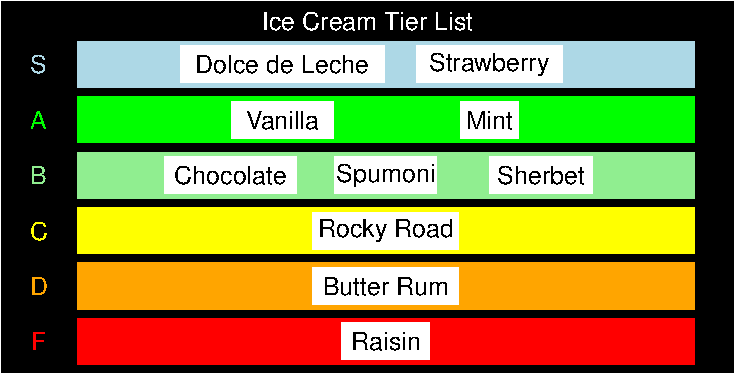
\includegraphics{Assignment1_Rcode_files/figure-latex/unnamed-chunk-3-1.pdf}

\newpage

\section{Part 3 - Write a Four-way Venn Diagram function {[}16
marks{]}}\label{part-3---write-a-four-way-venn-diagram-function-16-marks}

A client wants a function to make a standard four-way Venn diagram, like
one of the following:

\begin{enumerate}
\def\labelenumi{\alph{enumi})}
\tightlist
\item
  (8 marks) Make a function called \texttt{venn.oval} using the
  following code as a starting point. This function should draw an oval
  with the following parameters:
\end{enumerate}

\begin{itemize}
\tightlist
\item
  Take in a set of center xy coordinates, a long axis xy coordinates, a
  short axis xy coordinates, and a fill colour.
\item
  Create a convex \texttt{polygon()} of 8 sides that resembles an oval,
  that is symmetric along the long axis (from centerxy to longxy) and
  the short axis (from centerxy to shortxy)
\item
  The oval should not simply be a diamond, that would be four sides.
\end{itemize}

\begin{Shaded}
\begin{Highlighting}[]
\NormalTok{venn.oval }\OtherTok{=} \ControlFlowTok{function}\NormalTok{(}\AttributeTok{centerxy =} \FunctionTok{c}\NormalTok{(}\DecValTok{0}\NormalTok{,}\DecValTok{0}\NormalTok{), }\AttributeTok{longxy =} \FunctionTok{c}\NormalTok{(}\DecValTok{2}\NormalTok{,}\SpecialCharTok{{-}}\DecValTok{2}\NormalTok{), }
                 \AttributeTok{shortxy =} \FunctionTok{c}\NormalTok{(}\DecValTok{1}\NormalTok{,}\DecValTok{1}\NormalTok{), }\AttributeTok{col=}\StringTok{"\#FFFFFF"}\NormalTok{)}
\NormalTok{\{}
\CommentTok{\# We can use the mathematical function for an ellipse to use in Venn diagram }

\NormalTok{h }\OtherTok{\textless{}{-}}\NormalTok{ centerxy[}\DecValTok{1}\NormalTok{]  }\CommentTok{\# Center x}
\NormalTok{k }\OtherTok{\textless{}{-}}\NormalTok{ centerxy[}\DecValTok{2}\NormalTok{]  }\CommentTok{\# Center y}
\NormalTok{a }\OtherTok{\textless{}{-}} \DecValTok{3}  \CommentTok{\# Semi{-}major axis (long)}
\NormalTok{b }\OtherTok{\textless{}{-}} \DecValTok{2}  \CommentTok{\# Semi{-}minor axis (short)}
\NormalTok{angle }\OtherTok{\textless{}{-}} \DecValTok{65} \SpecialCharTok{*}\NormalTok{(pi}\SpecialCharTok{/}\DecValTok{180}\NormalTok{) }\CommentTok{\# Angle of the ellipse}

\CommentTok{\# Generate ellipse points using mathematic function of a ellipse}
\NormalTok{t }\OtherTok{\textless{}{-}} \FunctionTok{seq}\NormalTok{(}\DecValTok{0}\NormalTok{, }\DecValTok{2}\SpecialCharTok{*}\NormalTok{pi, }\AttributeTok{length.out =} \DecValTok{100}\NormalTok{)}
\NormalTok{x }\OtherTok{\textless{}{-}}\NormalTok{ h }\SpecialCharTok{+}\NormalTok{ a }\SpecialCharTok{*} \FunctionTok{cos}\NormalTok{(t) }\SpecialCharTok{*} \FunctionTok{cos}\NormalTok{(angle) }\SpecialCharTok{{-}}\NormalTok{ b }\SpecialCharTok{*} \FunctionTok{sin}\NormalTok{(t) }\SpecialCharTok{*} \FunctionTok{sin}\NormalTok{(angle)}
\NormalTok{y }\OtherTok{\textless{}{-}}\NormalTok{ k }\SpecialCharTok{+}\NormalTok{ a }\SpecialCharTok{*} \FunctionTok{cos}\NormalTok{(t) }\SpecialCharTok{*} \FunctionTok{sin}\NormalTok{(angle) }\SpecialCharTok{+}\NormalTok{ b }\SpecialCharTok{*} \FunctionTok{sin}\NormalTok{(t) }\SpecialCharTok{*} \FunctionTok{cos}\NormalTok{(angle)}
\FunctionTok{polygon}\NormalTok{(x, y)}
\NormalTok{  \}}
\end{Highlighting}
\end{Shaded}

Test the function with the following code

\begin{Shaded}
\begin{Highlighting}[]
\FunctionTok{plot.new}\NormalTok{()}
\FunctionTok{plot.window}\NormalTok{(}\AttributeTok{xlim=}\FunctionTok{c}\NormalTok{(}\SpecialCharTok{{-}}\DecValTok{5}\NormalTok{,}\DecValTok{5}\NormalTok{), }\AttributeTok{ylim=}\FunctionTok{c}\NormalTok{(}\SpecialCharTok{{-}}\DecValTok{5}\NormalTok{,}\DecValTok{5}\NormalTok{))}
\FunctionTok{venn.oval}\NormalTok{(}\AttributeTok{centerxy =} \FunctionTok{c}\NormalTok{(}\DecValTok{0}\NormalTok{,}\DecValTok{0}\NormalTok{), }\AttributeTok{longxy =} \FunctionTok{c}\NormalTok{(}\DecValTok{2}\NormalTok{,}\SpecialCharTok{{-}}\DecValTok{2}\NormalTok{), }
                 \AttributeTok{shortxy =} \FunctionTok{c}\NormalTok{(}\DecValTok{1}\NormalTok{,}\DecValTok{1}\NormalTok{), }\AttributeTok{col=}\StringTok{"\#FFFFFF"}\NormalTok{)}
\end{Highlighting}
\end{Shaded}

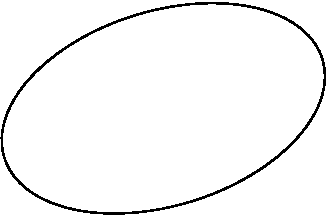
\includegraphics{Assignment1_Rcode_files/figure-latex/unnamed-chunk-5-1.pdf}

\begin{enumerate}
\def\labelenumi{\alph{enumi})}
\setcounter{enumi}{1}
\tightlist
\item
  (4 marks) Make a four-way venn diagram function called \texttt{venn4}.
  The function should take in the following parameters:
\end{enumerate}

\begin{itemize}
\tightlist
\item
  Call \texttt{venn.oval} four times, using the colours Cyan, Magenta,
  Yellow, and Black, all at 80/255 opacity.
\item
  Use the hex codes for the colours
\item
  Be arranged in such a way that all 16 possible overlaps (include `none
  of the four ovals' and `all of the four ovals') are on the screen.
\end{itemize}

\begin{Shaded}
\begin{Highlighting}[]
\NormalTok{venn4 }\OtherTok{=} \ControlFlowTok{function}\NormalTok{(}\AttributeTok{centerx =} \FunctionTok{c}\NormalTok{(}\SpecialCharTok{{-}}\DecValTok{1}\NormalTok{,}\DecValTok{0}\NormalTok{,}\DecValTok{2}\NormalTok{,}\DecValTok{3}\NormalTok{), }
                 \AttributeTok{centery =} \FunctionTok{c}\NormalTok{(}\DecValTok{0}\NormalTok{,}\DecValTok{1}\NormalTok{,}\DecValTok{1}\NormalTok{,}\DecValTok{0}\NormalTok{), }
                 \AttributeTok{cols =} \FunctionTok{rep}\NormalTok{(}\StringTok{"\#FFFFFF"}\NormalTok{, }\DecValTok{4}\NormalTok{), }
                 \AttributeTok{angle =} \FunctionTok{c}\NormalTok{(}\DecValTok{0}\NormalTok{,}\DecValTok{0}\NormalTok{,}\DecValTok{0}\NormalTok{,}\DecValTok{0}\NormalTok{ )) \{   }
  
\NormalTok{  angle }\OtherTok{\textless{}{-}}\NormalTok{ angle }\SpecialCharTok{*}\NormalTok{ pi }\SpecialCharTok{/} \DecValTok{180}  \CommentTok{\# Convert degrees to radians}

  \ControlFlowTok{for}\NormalTok{ (i }\ControlFlowTok{in} \DecValTok{1}\SpecialCharTok{:}\FunctionTok{length}\NormalTok{(centerx)) \{}
\NormalTok{    h }\OtherTok{\textless{}{-}}\NormalTok{ centerx[i]  }\CommentTok{\# Center x}
\NormalTok{    k }\OtherTok{\textless{}{-}}\NormalTok{ centery[i]  }\CommentTok{\# Center y}
\NormalTok{    a }\OtherTok{\textless{}{-}} \DecValTok{2}  \CommentTok{\# Semi{-}major axis (long)}
\NormalTok{    b }\OtherTok{\textless{}{-}} \DecValTok{1}  \CommentTok{\# Semi{-}minor axis (short)}
\NormalTok{    theta }\OtherTok{\textless{}{-}}\NormalTok{ angle[i]  }\CommentTok{\# Correct angle for this ellipse}

    \CommentTok{\# Generate ellipse points without rotation}
\NormalTok{    t }\OtherTok{\textless{}{-}} \FunctionTok{seq}\NormalTok{(}\DecValTok{0}\NormalTok{, }\DecValTok{2}\SpecialCharTok{*}\NormalTok{pi, }\AttributeTok{length.out =} \DecValTok{100}\NormalTok{)}
\NormalTok{    x\_ellipse }\OtherTok{\textless{}{-}}\NormalTok{ a }\SpecialCharTok{*} \FunctionTok{cos}\NormalTok{(t)  }\CommentTok{\# Standard ellipse x{-}coordinates}
\NormalTok{    y\_ellipse }\OtherTok{\textless{}{-}}\NormalTok{ b }\SpecialCharTok{*} \FunctionTok{sin}\NormalTok{(t)  }\CommentTok{\# Standard ellipse y{-}coordinates}
    
    \CommentTok{\# Apply rotation transformation}
\NormalTok{    x }\OtherTok{\textless{}{-}}\NormalTok{ h }\SpecialCharTok{+}\NormalTok{ x\_ellipse }\SpecialCharTok{*} \FunctionTok{cos}\NormalTok{(theta) }\SpecialCharTok{{-}}\NormalTok{ y\_ellipse }\SpecialCharTok{*} \FunctionTok{sin}\NormalTok{(theta)}
\NormalTok{    y }\OtherTok{\textless{}{-}}\NormalTok{ k }\SpecialCharTok{+}\NormalTok{ x\_ellipse }\SpecialCharTok{*} \FunctionTok{sin}\NormalTok{(theta) }\SpecialCharTok{+}\NormalTok{ y\_ellipse }\SpecialCharTok{*} \FunctionTok{cos}\NormalTok{(theta)}
  
    \CommentTok{\# Plot each ellipse}
    \FunctionTok{polygon}\NormalTok{(x, y, }\AttributeTok{col =} \FunctionTok{adjustcolor}\NormalTok{(cols[i], }\AttributeTok{alpha =} \FloatTok{0.5}\NormalTok{), }\AttributeTok{border =}\NormalTok{ cols[i])}
\NormalTok{  \}   }
\NormalTok{\}}
\end{Highlighting}
\end{Shaded}

Test your function with the following code

\begin{Shaded}
\begin{Highlighting}[]
\FunctionTok{plot.new}\NormalTok{()}
\FunctionTok{plot.window}\NormalTok{(}\AttributeTok{xlim=}\FunctionTok{c}\NormalTok{(}\SpecialCharTok{{-}}\DecValTok{5}\NormalTok{,}\DecValTok{5}\NormalTok{), }\AttributeTok{ylim=}\FunctionTok{c}\NormalTok{(}\SpecialCharTok{{-}}\DecValTok{5}\NormalTok{,}\DecValTok{5}\NormalTok{))}

\FunctionTok{venn4}\NormalTok{(}\AttributeTok{centerx =} \FunctionTok{c}\NormalTok{(}\SpecialCharTok{{-}}\DecValTok{1}\NormalTok{,}\SpecialCharTok{{-}}\FloatTok{0.25}\NormalTok{,}\FloatTok{0.25}\NormalTok{,}\DecValTok{1}\NormalTok{), }
      \AttributeTok{centery =} \FunctionTok{c}\NormalTok{(}\DecValTok{0}\NormalTok{,}\DecValTok{1}\NormalTok{,}\DecValTok{1}\NormalTok{,}\DecValTok{0}\NormalTok{), }
      \AttributeTok{cols =} \FunctionTok{c}\NormalTok{(}\StringTok{"\#00FFFF"}\NormalTok{, }\StringTok{"\#FF00FF"}\NormalTok{, }\StringTok{"\#FFFF00"}\NormalTok{, }\StringTok{"\#000000"}\NormalTok{), }
     \AttributeTok{angle =} \FunctionTok{c}\NormalTok{(}\SpecialCharTok{{-}}\DecValTok{60}\NormalTok{,}\SpecialCharTok{{-}}\DecValTok{60}\NormalTok{,}\DecValTok{60}\NormalTok{,}\DecValTok{60}\NormalTok{))}
\end{Highlighting}
\end{Shaded}

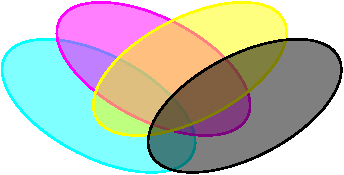
\includegraphics{Assignment1_Rcode_files/figure-latex/unnamed-chunk-7-1.pdf}

\end{document}
